\documentclass[11pt]{article}\usepackage[]{graphicx}\usepackage[]{color}
%% maxwidth is the original width if it is less than linewidth
%% otherwise use linewidth (to make sure the graphics do not exceed the margin)
\makeatletter
\def\maxwidth{ %
  \ifdim\Gin@nat@width>\linewidth
    \linewidth
  \else
    \Gin@nat@width
  \fi
}
\makeatother
\usepackage{pdfpages} 
\definecolor{fgcolor}{rgb}{0.345, 0.345, 0.345}
\newcommand{\hlnum}[1]{\textcolor[rgb]{0.686,0.059,0.569}{#1}}%
\newcommand{\hlstr}[1]{\textcolor[rgb]{0.192,0.494,0.8}{#1}}%
\newcommand{\hlcom}[1]{\textcolor[rgb]{0.678,0.584,0.686}{\textit{#1}}}%
\newcommand{\hlopt}[1]{\textcolor[rgb]{0,0,0}{#1}}%
\newcommand{\hlstd}[1]{\textcolor[rgb]{0.345,0.345,0.345}{#1}}%
\newcommand{\hlkwa}[1]{\textcolor[rgb]{0.161,0.373,0.58}{\textbf{#1}}}%
\newcommand{\hlkwb}[1]{\textcolor[rgb]{0.69,0.353,0.396}{#1}}%
\newcommand{\hlkwc}[1]{\textcolor[rgb]{0.333,0.667,0.333}{#1}}%
\newcommand{\hlkwd}[1]{\textcolor[rgb]{0.737,0.353,0.396}{\textbf{#1}}}%
\let\hlipl\hlkwb

\usepackage{ulem}

\usepackage{framed}
\makeatletter
\newenvironment{kframe}{%
 \def\at@end@of@kframe{}%
 \ifinner\ifhmode%
  \def\at@end@of@kframe{\end{minipage}}%
  \begin{minipage}{\columnwidth}%
 \fi\fi%
 \def\FrameCommand##1{\hskip\@totalleftmargin \hskip-\fboxsep
 \colorbox{shadecolor}{##1}\hskip-\fboxsep
     % There is no \\@totalrightmargin, so:
     \hskip-\linewidth \hskip-\@totalleftmargin \hskip\columnwidth}%
 \MakeFramed {\advance\hsize-\width
   \@totalleftmargin\z@ \linewidth\hsize
   \@setminipage}}%
 {\par\unskip\endMakeFramed%
 \at@end@of@kframe}
\makeatother

\definecolor{shadecolor}{rgb}{.97, .97, .97}
\definecolor{messagecolor}{rgb}{0, 0, 0}
\definecolor{warningcolor}{rgb}{1, 0, 1}
\definecolor{errorcolor}{rgb}{1, 0, 0}
\newenvironment{knitrout}{}{} % an empty environment to be redefined in TeX

\usepackage{alltt}
\usepackage{graphicx, fancyhdr}
\usepackage{amsmath, amsfonts}
\usepackage{color}
\usepackage{hyperref}
\usepackage{capt-of}
\newcommand{\blue}[1]{{\color{blue} #1}}

\setlength{\topmargin}{-.5 in} 
\setlength{\textheight}{9 in}
\setlength{\textwidth}{6.5 in} 
\setlength{\evensidemargin}{0 in}
\setlength{\oddsidemargin}{0 in} 
\setlength{\parindent}{0 in}
\newcommand{\ben}{\begin{enumerate}}
\newcommand{\een}{\end{enumerate}}


\lhead{STAT 305}
\chead{Homework \# 3} 
\rhead{Solution }
\lfoot{Fall 2019} 
\cfoot{\thepage} 
\rfoot{} 
\renewcommand{\headrulewidth}{0.4pt} 
\renewcommand{\footrulewidth}{0.4pt} 

\def\Exp#1#2{\ensuremath{#1\times 10^{#2}}}
\def\Case#1#2#3#4{\left\{ \begin{tabular}{cc} #1 & #2 \phantom
{\Big|} \\ #3 & #4 \phantom{\Big|} \end{tabular} \right.}
\IfFileExists{upquote.sty}{\usepackage{upquote}}{}
\begin{document}
\pagestyle{fancy} 
\begin{itemize}
\item \textbf{Problem 1:} \\ % chapter 3 section 2 problem 2 page 92
(a) Provide a QQ-plot for the two data sets below. \textbf{Note:} Be careful about the size of the two data sets. [10 pts] \\
\textbf{Solution:}\\
\begin{center}
	\begin{minipage}{\linewidth}
		\centering
		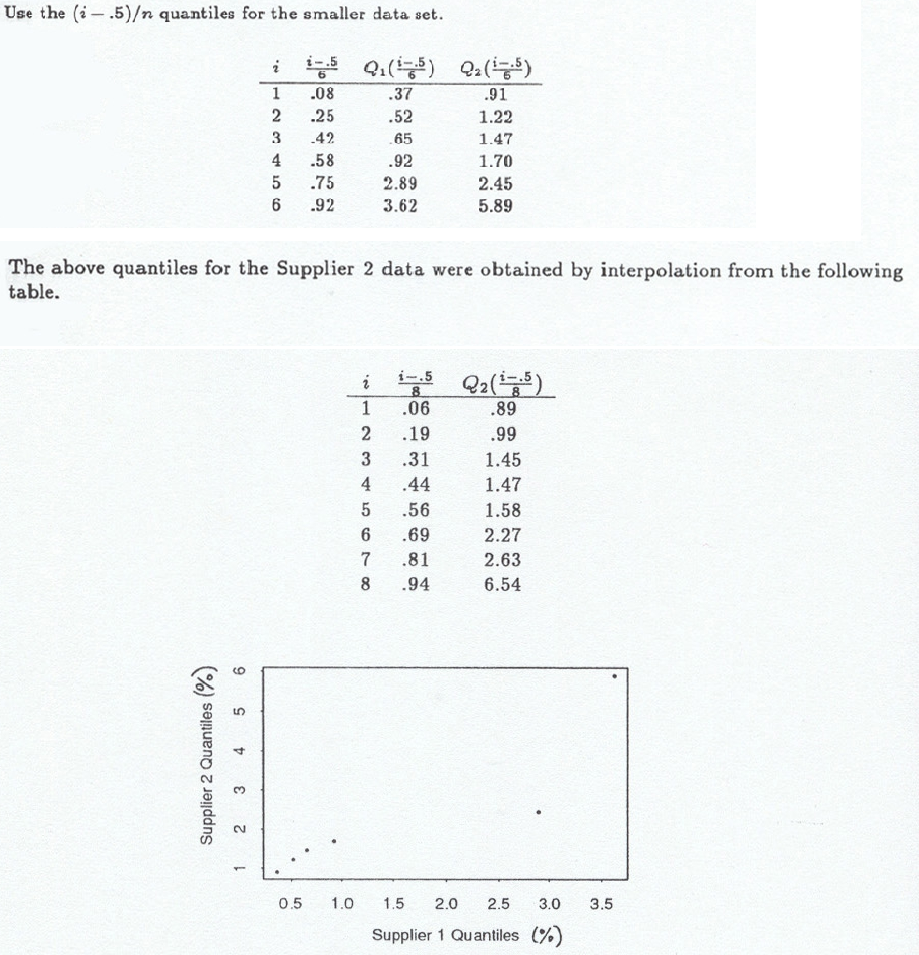
\includegraphics[width=\textwidth]{hw3p1.png}
	%	\captionof{figure}{Messung 1: Diagramm}
	\end{minipage}
\end{center}

(b) What can you say about the shape of the two data sets? [5 pts]\\
\textbf{Solution:} It seems the data of the two supliers have \textbf{ the same shape} (except one  quantile at $(2.89, 2.45)$. 

\item \textbf{Problem 2:} (a) Explain the usefulness of theoretical QQ-plots  [5 pts]\\
%chapter 3 section 2 page 92 problem 4
\textbf{Sulotion:} Theoretical QQ-plotting allows you to roughly check to see if \textbf{a data set has s shape which is similar to some theoretical distribution.} This can be useful in \textbf{identifying a theoretical (probability) model to represent how the process is generating data. } Such a model can be then used to make inferences (conclusions) about the process. \\

(b) There is an excel file named "ballbearings.csv" as the relevant material of homework 3 on the course page \href{https://ashirazist.github.io/stat305.github.io/homework.html}{(here)}. Use JMP to draw a Normal probability plot for \textbf{Group1} and \textbf{Group2} in the excel file separately.(You may use the tutorial, and just copy and paste the two QQ-plots)[5 pts for each plot] \\
\textbf{Solution:} For Group I, the Normal QQ-plot is
\begin{center}
	\begin{minipage}{\linewidth}
		\centering
		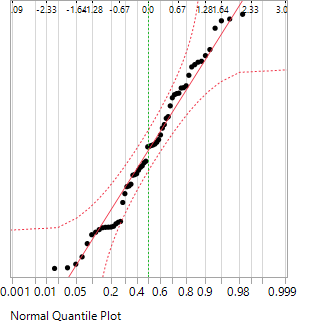
\includegraphics[width=6cm, height=6cm]{hw3p2b1.png}
		%	\captionof{figure}{Messung 1: Diagramm}
	\end{minipage}
\end{center}
and for Group II:
\begin{center}
	\begin{minipage}{\linewidth}
		\centering
		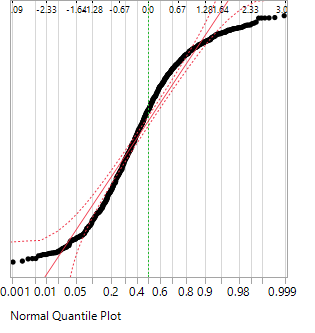
\includegraphics[width=6cm, height=6cm]{hw3p2b2.png}
		%	\captionof{figure}{Messung 1: Diagramm}
	\end{minipage}
\end{center}
(c) Comment on the two QQ-plots you draw in part (b) of how similar the shapes of the data are to the theoretical quantile of Normal distribution and explain why.[10 pts]\\
The answer to the question is that the two data set \textbf{DO NOT HAVE SIMILAR SHAPE WITH THE NORMAL DISTRIBUTION.} The reason is that the QQ-plot of the two Groups of the data do not lie around the straight line in the QQ-plot of Normal distribution.( you get the full credit for answers close to this); however, you might come with the discussion that the two data sets are somehow similar to Normal distribution in shape except the extreme quantiles, especially for Group I where the data lie around the straight line better than Group II. 


\item \textbf{Problem 3:}   End Chapter Exercise, Problem 9 (page 116)  [part (a) 10 pts- part (b) 5 pts ]. \\
\textbf{Note:} Summarizing the data means you should find the sample mean, sample standard deviation, median, IQR and range of the data. Then draw appropriate plots to discuss the distributional shape of the data\\
 \textbf{Solution:}\\
 \begin{center}
 	\begin{minipage}{\linewidth}
 		\centering
 		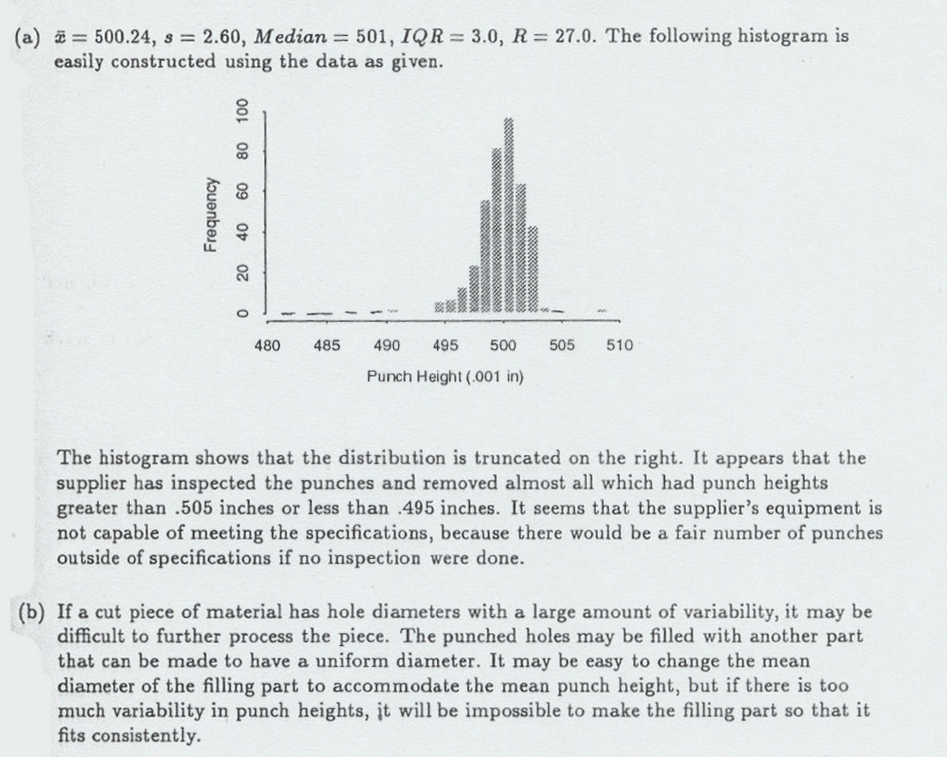
\includegraphics[width=\textwidth]{hw3p3.png}
 		%	\captionof{figure}{Messung 1: Diagramm}
 	\end{minipage}
 \end{center}

\item \textbf{Problem 4:} There is a study with 5 factors, each with 3 levels, how many observations do we need to have a \textit{ full factorial study}? [5 pts]\\
\textbf{Solution:}
$3^{5}= 243$\\

 \textbf{Note:} If the factors in a design all have the same number of levels, all possible combinations for a full factorial study has $$(\# of\  levels )^{(\# of\  factors)}$$

\item \textbf{Problem 5: }Frequently, several measurements of a quantity are made
	under similar conditions using a single measuring device and are
	then averaged to produce a final value. Which of the aspects of
	measurement  can be improved by this measurement and averaging process?. [5 pts] \\
\textbf{Solution:} Accuracy (or unbiasness) is how close a measurement is to the true value "on average"
%\item \textbf{Problem 6:}  An engineer woke up in the middle of the night, struck with the sudden awareness that when reporting the standard deviation for a recent sample of safety criteria tests, she mistakenly used the population formula, replacing $\mu$ with $\bar{x}$, instead of the correct sample formula. \\
%	\begin{enumerate}
	
%	\item Was the value for standard deviation she reported too large or too small? Explain.[5 pts]
	
%	\item Write the ratio of the formula she used (population standard deviation, with $\mu$ replaced by $\bar{x}$) to the formula she should have used (sample standard deviation). Simplify it as much as possible (note: it should only depend on sample size).[10 pts]
	
%	\item What happens to this ratio you if the sample size is very large? What happens as the sample size goes to infinity?[5 pts]
	
%\end{enumerate} 


\item \textbf{Problem 6:} Calculate the variance for the following samples (\textit{note: if you are neat with your work, you may notice a pattern}):[3 pts each]
\begin{enumerate}
	\item Sample 1: -1.05, -1.0, -0.5, 0.15, 0.6, 0.65, 0.7, 1.25\\
	
	\begin{align*}
	\bar{x} &= \frac{1}{n}\sum_{i=1}^{n}x_i\\
			&= \frac{1}{8}\sum_{i=1}^{8}x_i= \frac{1}{8} (-1.05 + (-1.0)+ (-0.5) + 0.15 + 0.6 + 0.65+ 0.7+ 1.25) \\
			&= 0.1\\
	s^2 &= \frac{1}{n-1}\sum_{i=1}^5 (x_i - \bar{x})^2 \\
		&= \frac{1}{n-1}( (x_1 - \bar{x})^2 + (x_2 - \bar{x})^2 + (x_3 - \bar{x})^2 + (x_4 - \bar{x})^2 + (x_5 - \bar{x})^2+ (x_6 - \bar{x})^2+ (x_7 - \bar{x})^2\\
		&+ (x_8 - \bar{x})^2  )\\
		&= \frac{1}{8}( (-1.05 -0.1)^2 + (-1.0 - 0.1)^2+ (-0.5 - 0.1)^2+ (0.15 - 0.1)^2+ (0.6 - 0.1)^2\\
		&+ (0.65 - 0.1)^2+ (0.7 - 0.1)^2+ (1.25 - 0.1)^2  )\\
		&= 0.73\\
	s&= \sqrt{s^2}= 0.85
	\end{align*}
	
	\item Sample 2: -2.1, -2.0, -1.0, 0.3, 1.2, 1.3, 1.4, 2.5\\
		\begin{align*}
	\bar{x} &= \frac{1}{n}\sum_{i=1}^{n}x_i\\
	&= \frac{1}{8}\sum_{i=1}^{8}x_i= \frac{1}{8} (-2.1+ (-2.0)+ (-1.0)+ 0.3+ 1.2+ 1.3+ 1.4+ 2.5) \\
	&= 0.2\\
	s^2 &= \frac{1}{n-1}\sum_{i=1}^5 (x_i - \bar{x})^2 \\
	&= \frac{1}{n-1}( (x_1 - \bar{x})^2 + (x_2 - \bar{x})^2 + (x_3 - \bar{x})^2 + (x_4 - \bar{x})^2 + (x_5 - \bar{x})^2+ (x_6 - \bar{x})^2+ (x_7 - \bar{x})^2\\
	&+ (x_8 - \bar{x})^2  )\\
	&= \frac{1}{8}( (-2.1 -0.2)^2 + ( -2.0 - 0.2)^2+ (-1.0 - 0.2)^2+ (0.3 - 0.2)^2+ (1.2 - 0.2)^2\\
	&+ (1.3 - 0.2)^2+ (1.4 - 0.2)^2+ (2.5 - 0.2)^2  )\\
	&= 2.93\\
	s&= \sqrt{s^2}= 1.71
	\end{align*}
	
	\item Sample 3: -4.2, -4.0, -2.0, 0.6, 2.4, 2.6, 2.8, 5.0\\
    \begin{align*}
	\bar{x} &= \frac{1}{n}\sum_{i=1}^{n}x_i\\
	&=  0.4\\
	s^2 &= \frac{1}{n-1}\sum_{i=1}^5 (x_i - \bar{x})^2 \\
	&= 11.72\\
	s&= \sqrt{s^2}= 3.42
	\end{align*}
	
	\item Sample 4: -8.4, -8.0, -4.0, 1.2, 4.8, 5.2, 5.6, 10.0\\
    \begin{align*}
	\bar{x} &= \frac{1}{n}\sum_{i=1}^{n}x_i\\
			&=  0.8\\
			s^2 &= \frac{1}{n-1}\sum_{i=1}^5 (x_i - \bar{x})^2 \\
			&= 46.90\\
			s&= \sqrt{s^2}= 6.84
	\end{align*}
		
	\item Sample 5: -16.8, -16.0, -8.0, 2.4, 9.6, 10.4, 11.2, 20.0\\
	\begin{align*}
			\bar{x} &= \frac{1}{n}\sum_{i=1}^{n}x_i\\
			&=  1.6\\
			s^2 &= \frac{1}{n-1}\sum_{i=1}^5 (x_i - \bar{x})^2 \\
			&= 187.64\\
			s&= \sqrt{s^2}= 6.8413.69
	\end{align*}			
\end{enumerate}



\item \textbf{Problem 7:} Mechanical engineers were interested in studying the effects of 2 chemical compounds 
	(low Ca, high Ca) and 3 uni-axial pressure (P1, P2, P3) on metal bars lifetime. A total of 12 specimen were assigned to the possible combinations with two metal bars in each treatment. The lifetime of the bars were recorded after each run of the experiment. 
\begin{enumerate}
	\item How many possible combinations of $compound$ $\times{ pressure}$ are there available for a full factorial study? Draw a table for this design to get full credit.[5 pts]\\
	\textbf{Solution:} There are $2\times{3} = 6$ possible combinations for a full factorial study. The following table shows a full factorial study with two specimen per treatment.
	\begin{center}
			\begin{tabular}{|c|c|c|c|}
				\hline
				& P1 & P2 &P3\\
				\hline
				Low Ca & $||$ &$||$ &$||$ \\
				\hline
				High Ca &$||$ &$||$ & $||$\\
				\hline
			\end{tabular}
	\end{center}
	
	\item What is the response variable in this study?[2 pts]\\
	\textbf{Solution:} The response variable is the metal bars lifetime
	\item What are experimental variables in this study? [2 pts]\\
	\textbf{Solution:} The chemical compound and uni-axial pressure are the experimental variables. 
	\item What type of experimental variables are they in part 3 above?(Be careful with this question, we already know they are experimental variables and not response variable)[2 pts]\\
	\textbf{Solution:} The chemical compound and uni-axial pressure are both \textbf{qualitative (categorical)} variables. 
	\item For this full factorial study with two factors chemical compounds and uni-axial pressure, the six experimental runs are labeled as:
	
	No. 1:  low- P1, \hspace{0.5cm} No. 2:  low-P2,
	\hspace{0.5cm} No. 3: low-P3, \\  No. 4:  high- P1,
	\hspace{0.5cm} No. 5:  high- P2, \hspace{0.1 cm}and
	\hspace{0.1cm} No. 6:  high- P3.
	
	\noindent Based on the following random digits
	
	\hspace{3.5cm}$49502 \; 18963 \; 63920 \; 39544 \; 25804$\\
	Which experiment should be done last?[4 pts]\\
	\textbf{Solution:} This exercise directly asks to use a random number table to randomly run the experiments. Using the digits, experimental run \textbf{NO. 3} will be the last to do. 
\end{enumerate}


	
Total: 95 pts


















\end{itemize}


\end{document}
